\newcommand{\decrease}[1]{\textsubscript{\textcolor{red}{$\downarrow$ #1}}}

\definecolor{highlightcolor}{HTML}{d4dcf7}
\begin{table}[t]
\caption{
Main results for SWE-agent performance on the full and Lite splits of the SWE-bench test set.
We benchmark models in the SWE-agent, Basic CLI, and Retrieval Augmented Generation (RAG) settings established in SWE-bench~\citep{jimenez2024swebench}.
}
\label{table:main-results}
\vspace{0.25em}
\centering
\begin{tabular}{lcccc}
    \toprule
    & \multicolumn{2}{c}{SWE-bench} & \multicolumn{2}{c}{SWE-bench Lite} \\
    \cmidrule(lr){2-3} \cmidrule(lr){4-5}
    Model & \% Resolved & \$ Avg. Cost & \% Resolved & \$ Avg. Cost \\
    \cmidrule(lr){1-1} \cmidrule(lr){2-3} \cmidrule(lr){4-5}
    RAG                        &             &      &             &      \\
    \smalltab w/ GPT-4 Turbo   &       1.31  & 0.13 &       2.67  & 0.13 \\
    \smalltab w/ Claude 3 Opus &       3.79  & 0.25 &       4.33  & 0.25 \\
    \cmidrule(lr){1-1}
    Shell-only agent                   &     &      &             &      \\
    \smalltab w/ GPT-4 Turbo           & -   & -    &      11.00  & 1.46 \\
    \smalltab\smalltab w/o Demonstration & -   & -   
    &       7.33  & 0.79 \\
    \cmidrule(lr){1-1}
    SWE-agent                  &             &      &             &      \\
    \smalltab w/ GPT-4 Turbo   & {\bf 12.47} & 1.59 & {\bf 18.00} & 1.67 \\
    \smalltab w/ Claude 3 Opus &      10.46  & 2.59 &      13.00  & 2.18 \\
    \bottomrule
\end{tabular}
% \end{table}

% \begin{table}
\renewcommand{\arraystretch}{1.1} % Adjust this value as needed
\begin{minipage}[b]{0.6\textwidth}
\caption{Pass@1 results on HumanEvalFix~\cite{muennighoff2023octopack}. Except for SWE-agent, we use scores as reported in~\citet{yu2023wavecoder}.}
\label{tab.benchmark_humanevalfix}
\vspace{0.25em}
\centering
\begin{tabular}{lcccc}
\toprule
    Model & Python & JS & Java \\
\midrule
    CodeLLaMa-instruct-13B & 29.2 & 19.5 & 32.3\\
    GPT-4 & 47.0 & 48.2 & 50.0 \\
    \small DeepseekCoder-CodeAlpaca-6.7B & 49.4 & 51.8 & 45.1 \\
    WaveCoder-DS-6.7B & 57.9 & 52.4 & 57.3 \\
    SWE-agent w/ GPT-4 Turbo & \textbf{87.7} & \textbf{89.7} & \textbf{87.9} \\
\bottomrule
\end{tabular}
\end{minipage}
\hfill
\begin{minipage}[b]{0.38\textwidth}
    \centering
    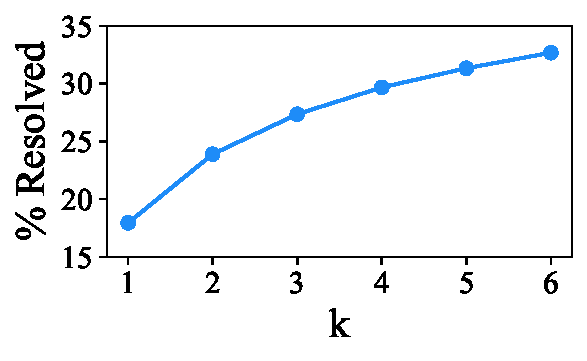
\includegraphics[width=\textwidth]{figures/pass_at_k.pdf}
    \captionof{figure}{
    SWE-agent w/ GPT-4 Turbo Pass$@k$ performance across \num{6} runs on SWE-bench Lite.
    }
    \label{fig:pass_at_k}
\end{minipage}

\centering
\caption{
SWE-bench Lite performance under ablations to the SWE-agent interface, which is denoted by \twemoji{cowboy_hat_face}. 
We consider different approaches to searching and editing (see Figures~\ref{fig.search.comparison} and \ref{fig.edit.comparison}, respectively).
We also verify how varying the file viewer window size affects performance, and we ablate the effect of different context management approaches.
}
\label{tab:combined_ablations_summary}
\vspace{0.25em}
{
\small
\begin{tabular}[t]{@{\hspace{0.05in}}l@{\hspace{0.07in}}l@{\hspace{0.05in}}}
    \toprule
    \multicolumn{2}{c}{\textbf{{Editor}}} \\
    \midrule
    \texttt{edit} action & 15.0  \decrease{3.0} \\
    \quad w/ linting \twemoji{cowboy_hat_face} & 18.0 \\
    No \texttt{edit} & 10.3 \decrease{7.7} \\
    \bottomrule
\end{tabular}
\hspace{0.05in}
\begin{tabular}[t]{@{\hspace{0.05in}}l@{\hspace{0.07in}}l@{\hspace{0.05in}}}
    \toprule
    \multicolumn{2}{c}{\textbf{{Search}}} \\
    \midrule
    Summarized \twemoji{cowboy_hat_face} & 18.0 \\
    Iterative & 12.0 \decrease{6.0} \\
    No search & 15.7 \decrease{2.3} \\
    \bottomrule
\end{tabular}
\hspace{0.05in}
\begin{tabular}[t]{@{\hspace{0.05in}}l@{\hspace{0.07in}}l@{\hspace{0.05in}}}
    \toprule
    \multicolumn{2}{c}{\textbf{{File Viewer}}} \\
    \midrule
    30 lines & 14.3 \decrease{3.7} \\
    100 lines \twemoji{cowboy_hat_face}  & 18.0 \\
    % 400 lines &  17.0 \decrease{1.0} \\
    Full file & 12.7 \decrease{5.3} \\
    \bottomrule
\end{tabular}
\hspace{0.05in}
\begin{tabular}[t]{@{\hspace{0.05in}}l@{\hspace{0.06in}}l@{\hspace{0.05in}}}
    \toprule
    \multicolumn{2}{c}{\textbf{{Context}}} \\
    \midrule
    Last 5 Obs. \twemoji{cowboy_hat_face}  & 18.0 \\
    Full history & 15.0 \decrease{3.0} \\
    w/o demo. & 16.3 \decrease{1.7} \\
    \bottomrule
\end{tabular}
}
\vspace{-3.5em}
\end{table}


\section{Results}
\label{sec:results}
Across all systems, SWE-agent w/ GPT-4 Turbo achieves the best performance all-around, successfully solving \num{12.47}\% (\num{286}/\num{2294}) of the full SWE-bench test set and \num{18.00}\% (\num{54}/\num{300}) of the Lite split.
As shown in Table~\ref{table:main-results}, compared to RAG on Lite, SWE-agent is \num{8}-\num{13}x more costly but yields a \num{6.7}-fold improved \% Resolved rate.
An LM-friendly ACI's value is confirmed by SWE-agent's \num{64}\% relative increase compared to Shell-only, both with GPT-4 Turbo.

In Table~\ref{tab.benchmark_humanevalfix}, SWE-agent yields strong performance on HumanEvalFix with \num{88.3}\% pass@1 rate.
Figure~\ref{fig:pass_at_k} reveals that average performance variance is relatively low, but per-instance resolution can change considerably.
More results are given in the appendix: \S\ref{appx:results:model_performance} shows that the success rate is uncorrelated to the issue age (controlling for possible test pollution), \ref{appx:analyses:pass_at_k} presents more details on performance variance and pass$@k$, and \ref{appx:analyses:additional_benchmarks} discusses extra evaluation details.

\subsection{Analysis of ACI Design}
\label{sec:analysis:interface-design}
We perform several ablations of the SWE-agent interface, specifically with respect to the SWE-agent w/ GPT-4 configuration, summarized in Table~\ref{tab:combined_ablations_summary}.
Our case studies shed light on interesting agent behavior along with the impact of different ACI designs.

\textbf{Human user interfaces are not always suitable as agent-computer interfaces.}
Current LMs are vulnerable to a number of pitfalls when searching for relevant content in a Linux shell environment.
Some exploration patterns (e.g., chains of \texttt{cd}, \texttt{ls}, \texttt{cat}) are extremely inefficient.
\texttt{grep} or \texttt{find} look ups can perform better but occasionally produce many lines of irrelevant results.
We hypothesize that better localization is possible with faster navigation and a more informative search interface. 

\begin{figure}[t]
\centering
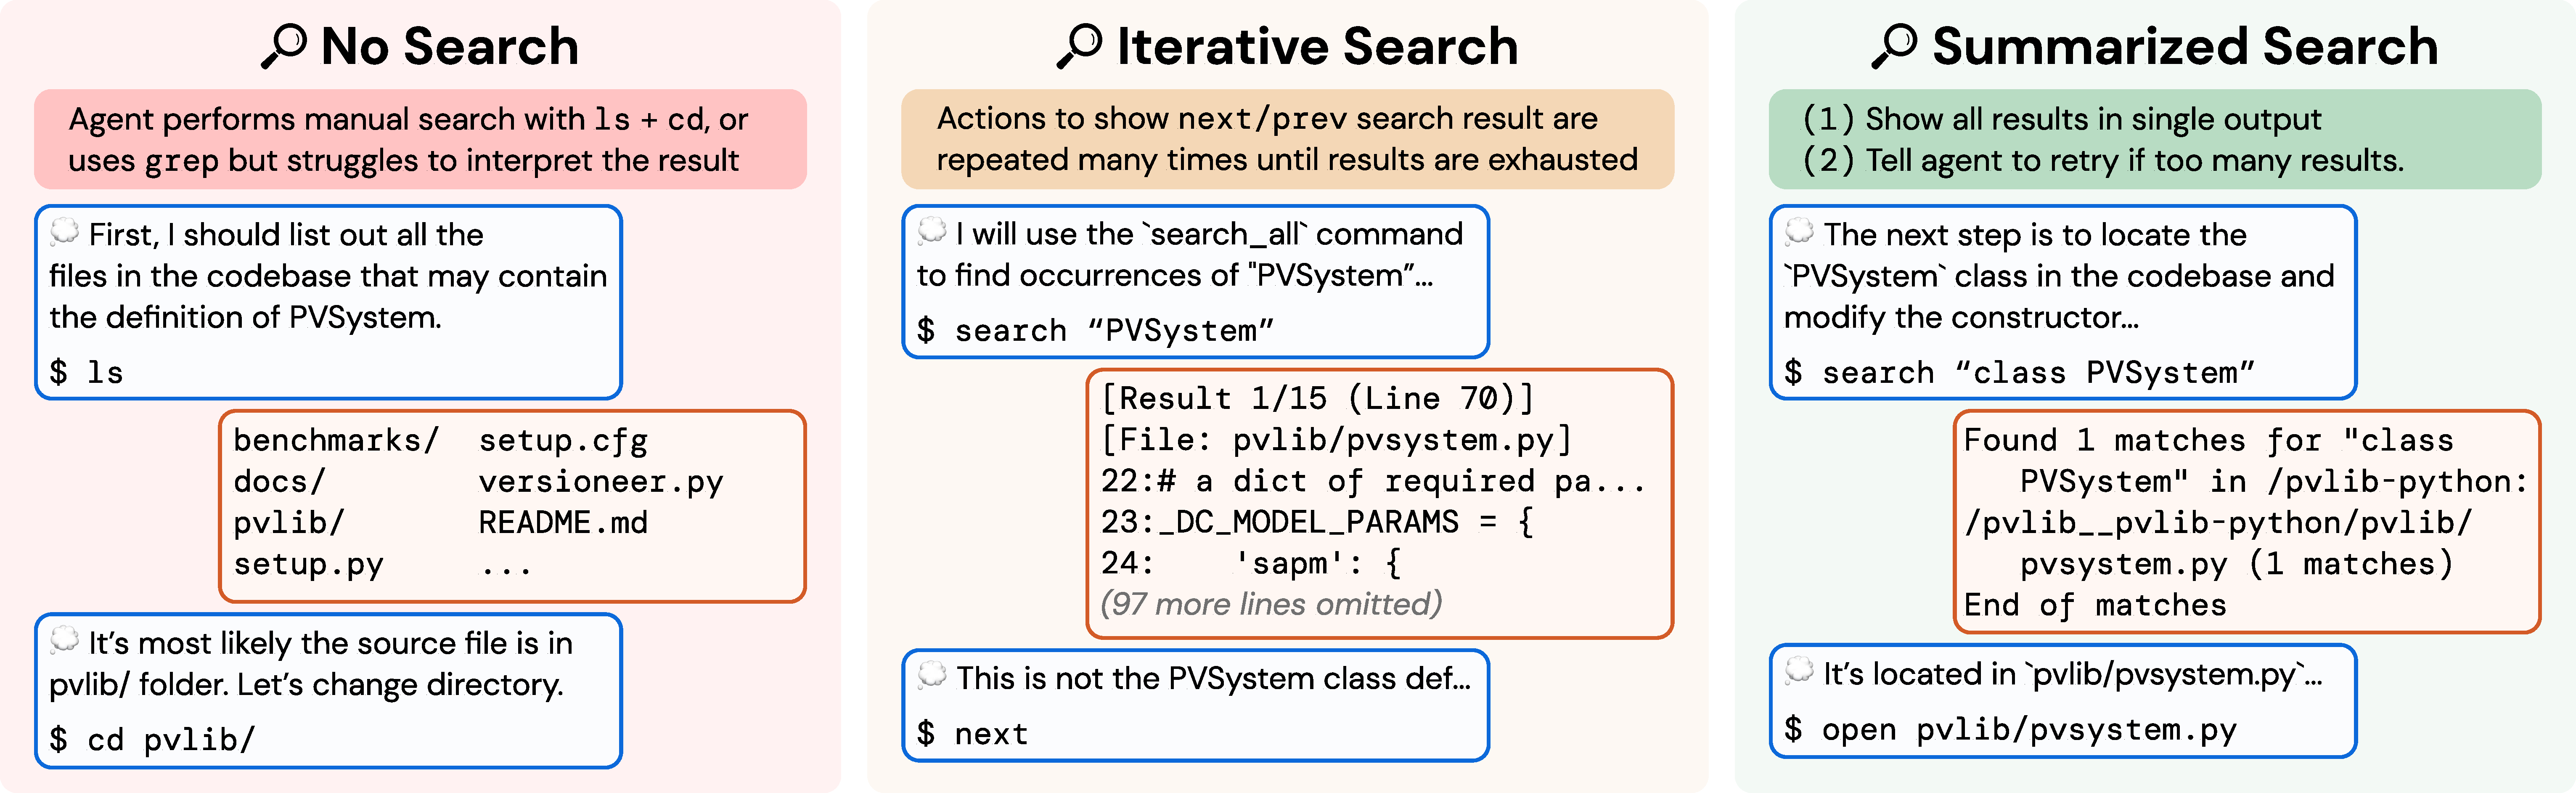
\includegraphics[width=\linewidth]{figures/search_comparison.pdf}
\caption{Three different Search interfaces for task instance \texttt{pvlib\_\_pvlib-python-1224}.
In Shell-only, an agent performs localization using only standard bash commands and utilities.
Compared to \textit{Iterative} search, \textit{Summarized} search shows an exhaustive list of search results and provides guidance on refining under-specified queries.}
\label{fig.search.comparison}
\vspace{1em}
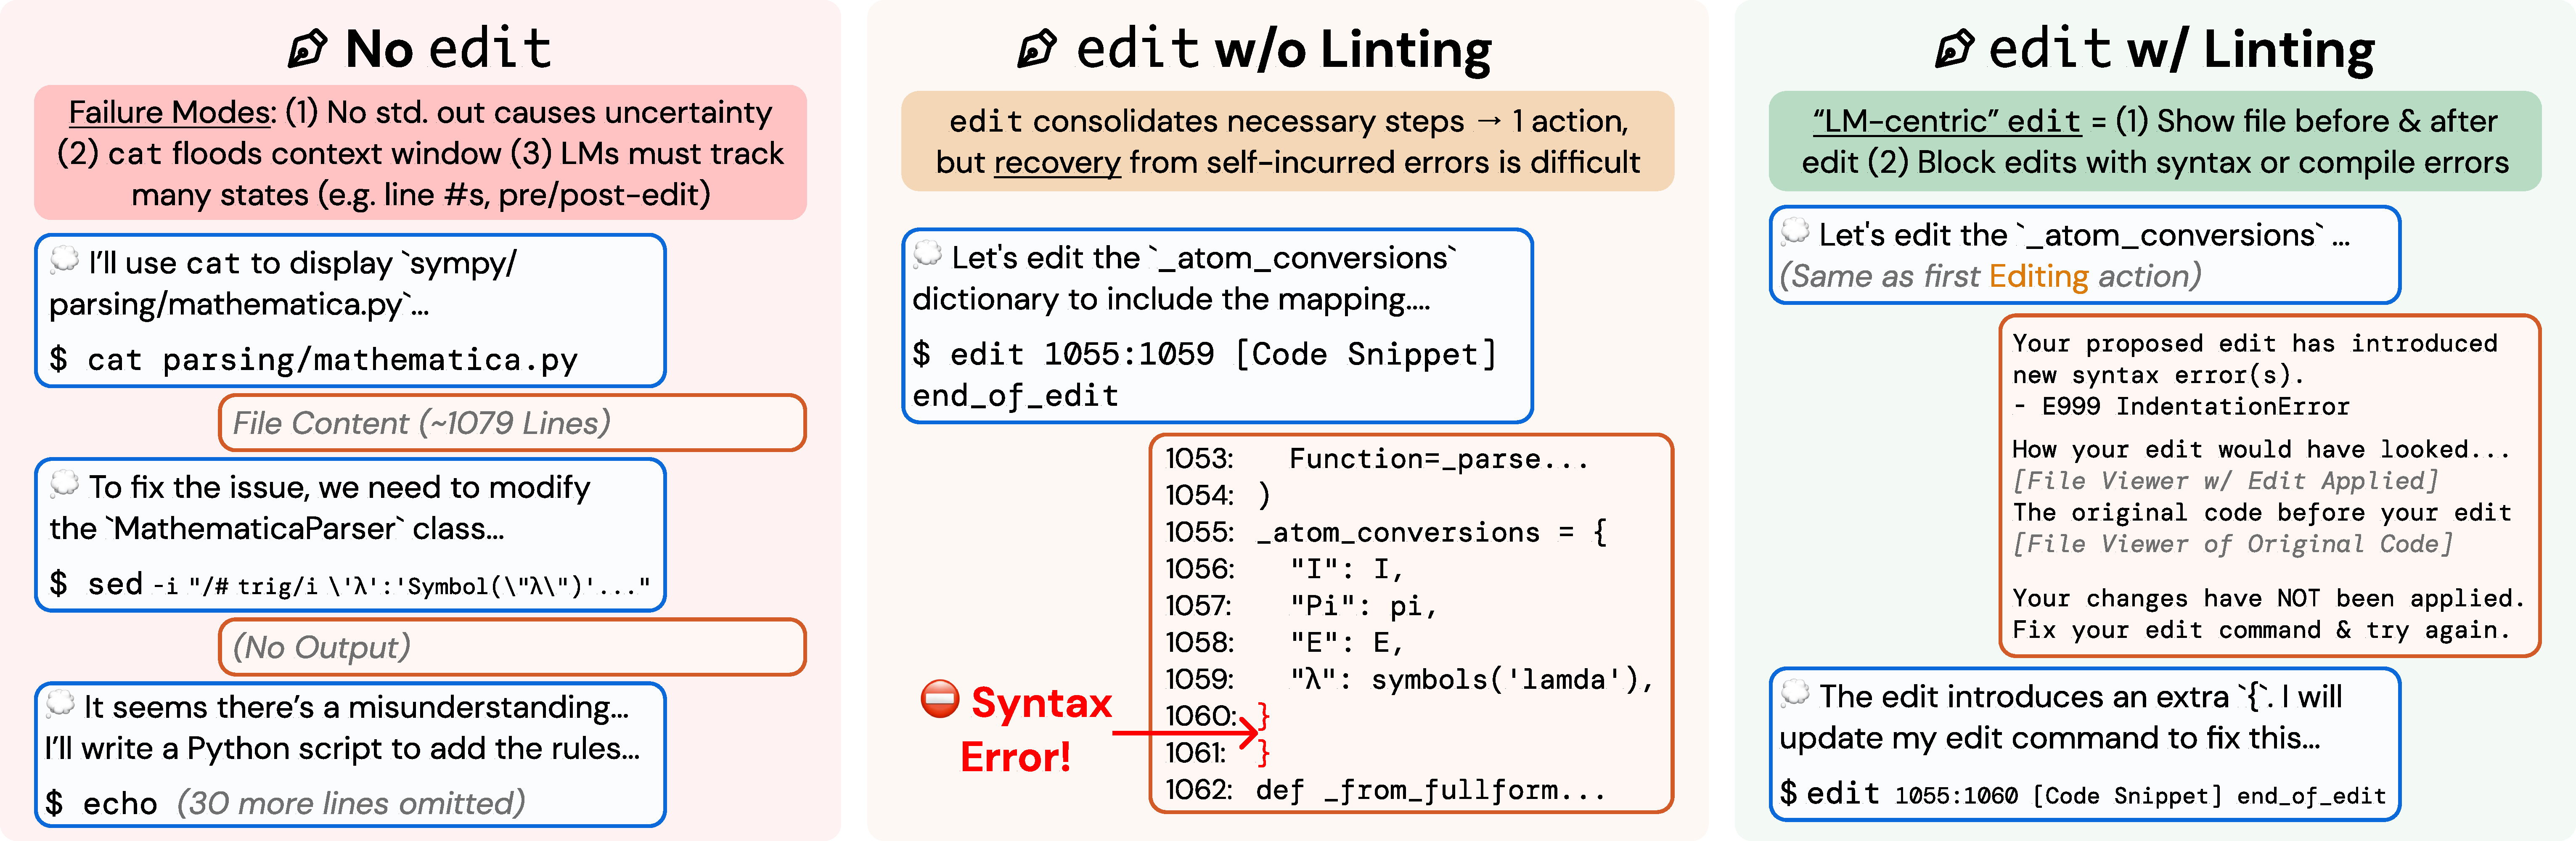
\includegraphics[width=\linewidth]{figures/edit_comparison.pdf}
\caption{Three different Edit interfaces for task instance \texttt{sympy\_\_sympy-24102}. Editing with bash commands requires several actions to successfully modify a file. The \textit{Editing} component defines an \texttt{edit} command that leverages the File Viewer component to replace the bash style of editing workflow with a single command. \textit{Linting} is beneficial for stymieing cascading errors that often start with an error-introducing edit by the agent.}
\label{fig.edit.comparison}
\end{figure}

Figure~\ref{fig.search.comparison} compares the Shell-only setting to  two different search interfaces.
\textit{Iterative} search, directly inspired by traditional user interfaces for search, e.g., \texttt{Vim} or VSCode, shows results one by one via the file viewer.
Agents can look through results using \texttt{next} and \texttt{prev} actions.
Each result displays the matching line along with \texttt{n} surrounding lines of context.
An advantage is that an agent can begin editing directly after seeing the relevant code in its search.
However, when given a large number of search results, agents tend to look through every match exhaustively, calling \texttt{next} until each result has been inspected.
This inefficient behavior can exhaust an agent's cost budget or context window, leading to even worse performance than the not having additional search tools at all (\num{15.7}\%\decrease{2.3} for No search vs. \num{12.0}\%\decrease{6.0} with Iterative search).

\textbf{Compact, efficient file editing is critical to performance.}
SWE-agent's file editor and viewer are designed to consolidate the editing process into a single command that enables easy multi-line edits with consistent feedback and automatically updates the agent's view of the file after editing.
In the No \texttt{edit} setting, editing options are restrictive and prone to errors; the primary methods available are either replacing entire files through redirection and overwriting or using utilities like \texttt{sed} for single-line or search-and-replace edits.
Both methods have significant drawbacks.
Redirection involves copying and rewriting entire files for even minor changes, which is both inefficient and error-prone.
Although \texttt{sed} can facilitate specific edits, executing multi-line edits is cumbersome and can lead to unintended consequences that are challenging to detect.
Moreover, both strategies lack immediate feedback about file updates, making these silent operations potentially confusing for models to interpret and increasing the risk of errors.
Without SWE-agent's file editor interface, performance drops to (\num{10.3}\% \decrease{7.7}).
We also find that agents are sensitive to the number of lines the file viewer displays.
Either too little content (30 lines, \num{14.3}\% \decrease{3.7}) or too much (entire file, \num{12.7}\% \decrease{5.3}) lowers performance.

\textbf{Guardrails can improve error recovery.}
A prominent failure mode occurs when models repeatedly \texttt{edit} the same code snippet.
The usual suspect for this behavior is an agent introducing a syntax error (e.g., incorrect indentation, extra parenthesis) via an errant \texttt{edit}.
As discussed in Section~\ref{sec:sweagent}, we add an intervention to the \texttt{edit} logic that lets a modification apply only if it does not produce major errors.
We compare this interface with the No \texttt{edit} and \texttt{edit} w/o linting alternatives  in Figure~\ref{fig.edit.comparison}.
This intervention improves performance considerably (without linting, \num{15.0}\% \decrease{3.0}).

\subsection{Analysis of Agent Behavior}
\label{sec:analysis:agent-behavior}
Recurring problem-solving patterns emerge when LMs are equipped with a useful, intuitive ACI.
We describe several model behaviors and problem-solving patterns that can be discerned from model performance and each model's corresponding trajectories.

\textbf{Reproduction and/or localization is the first step.}
SWE-agent usually begins with either writing reproduction code and/or localizing the issue's cause to specific lines of code.
As shown in Figure~\ref{fig:actions_per_turn}, all trajectories begin with either \texttt{create} (reproduction) or \texttt{find\_file}/\texttt{search\_dir} (localization).
To reproduce, models will \texttt{create} a new file, add reproduction code to it with an \texttt{edit}, then run with \texttt{python}; this is the most popular triple of actions in Table~\ref{tab:most_common_triples_by_index}.
Using this feedback along with file names and symbols in the issue description, an agent will start with a broad, directory-level keyword search, before then zooming into specific files and lines.
This is reflected in Figure~\ref{fig:transition_probs_2gram}, where the most likely actions following localization sequences like (\texttt{python}, \texttt{find\_file}) and (\texttt{search\_dir}, \texttt{open}) are \texttt{search\_file} and \texttt{goto}, indicative of how an agent ``zooms in" on a bug.
Extensive analysis on correlations between different groups of actions are discussed in \S\ref{appx:analyses:trajectory_analysis:action_breakdown}

\textbf{Remaining turns are mostly ``edit, then execute" loops.}
As exhibited in Figure~\ref{fig:actions_per_turn}, from turn \num{5} onwards, the most frequent two actions for all turns are \texttt{edit} and \texttt{python}.
Captured as high probability next actions following (\texttt{edit}, \texttt{python}) in Figure~\ref{fig:transition_probs_2gram}, additional localization operations are often interspersed across these later turns, where agents might look at more in-file code with \texttt{search\_file}, \texttt{scroll\_up/down}, or other files altogether with \texttt{search\_dir}, \texttt{find\_file}.
This behavior usually arises in response to new information from re-running the reproduction script.
Submissions are distributed normally from turn \num{10} onwards, although resolved task instances correlate more with earlier \texttt{submit}s (see \S\ref{appx:analyses:trajectory_analysis:turns_to_resolution}).
A walk-through of common trajectory phases is in \S\ref{appx:analyses:trajectory_analysis:walkthrough}.

\textbf{Editing remains challenging for agents.}
A non-trivial minority of edit actions raise a linting error; out of \num{2294} task instances, \num{1185} (\num{51.7}\%) of SWE-agent w/ GPT-4 Turbo trajectories have \num{1}+ failed edits.
While agents generally recover more often than not from failed edits, the odds of recovery decrease as the agent accumulates more failed edits.
Recovery refers to a sequence of consecutive failed edits followed immediately by a successful edit.
Any attempt at editing has a \num{90.5}\% chance of eventually being successful.
This probability drops off to \num{57.2}\% after a single failed edit.
More editing phenomena are discussed in \S\ref{appx:analyses:trajectory_analysis:action_breakdown}, and data about agents' generated fixes are in \S\ref{appx:analyses:patch_generations}.

\begin{figure}[t]
  \centering
  \begin{minipage}[t]{0.49\linewidth}
    \centering
    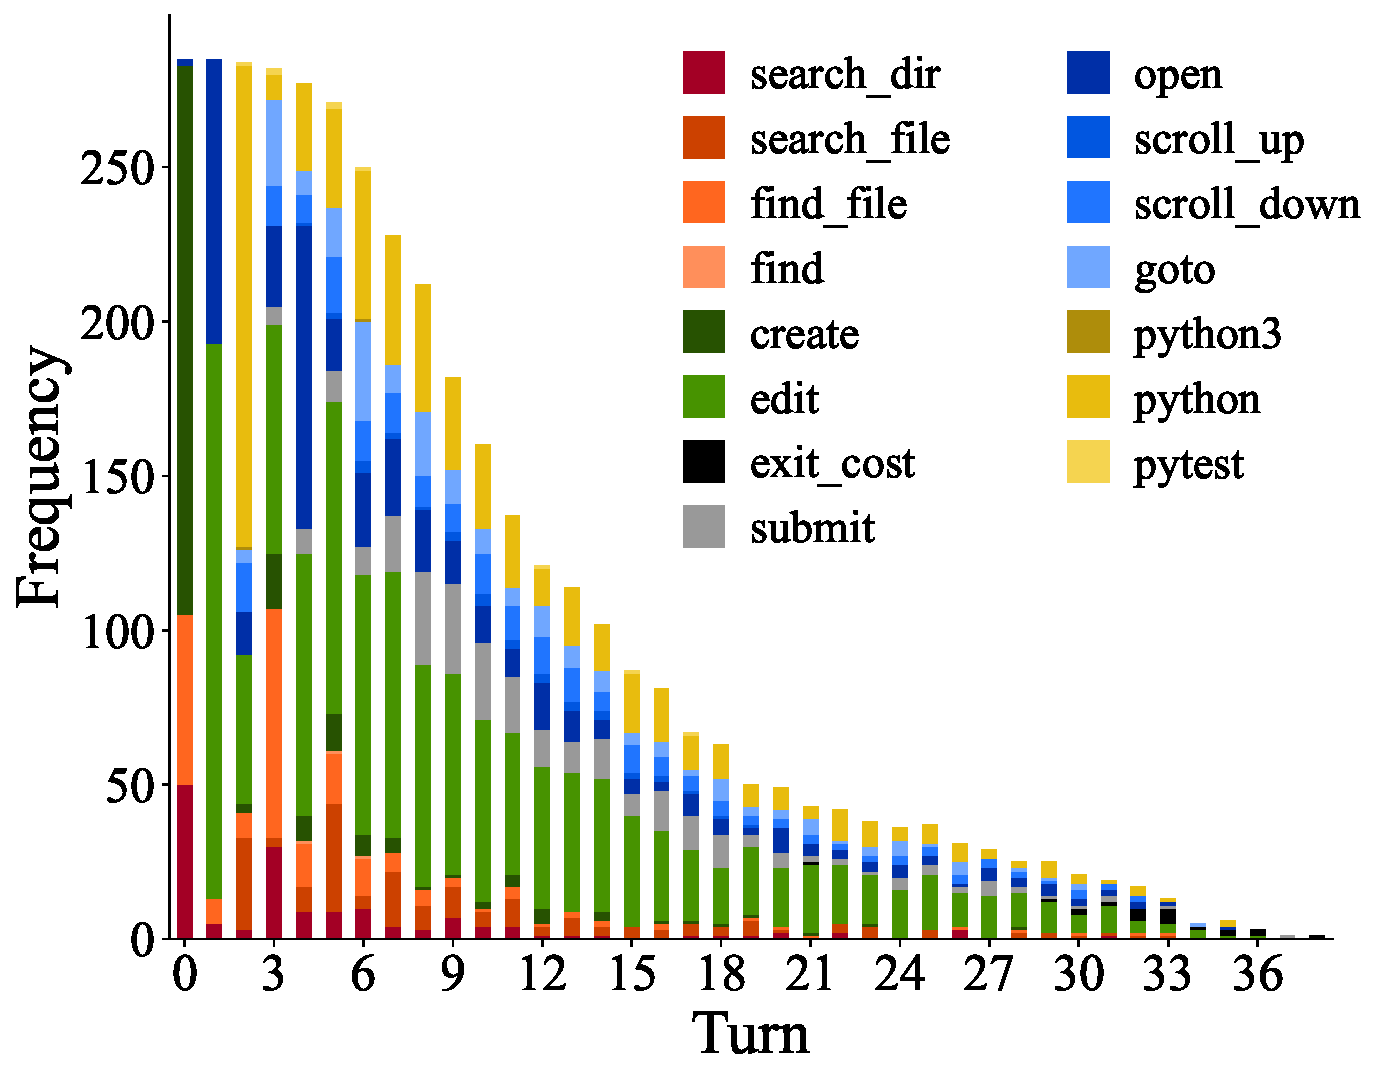
\includegraphics[width=\textwidth]{figures/actions_per_turn.pdf}
    \caption{The frequency with which actions are invoked at each turn by SWE-agent w/ GPT-4 for task instances that it solved on the SWE-bench full test set (\num{286} trajectories).}
    \label{fig:actions_per_turn}
  \end{minipage}
  \hfill
  \begin{minipage}[t]{0.49\linewidth}
    \centering
    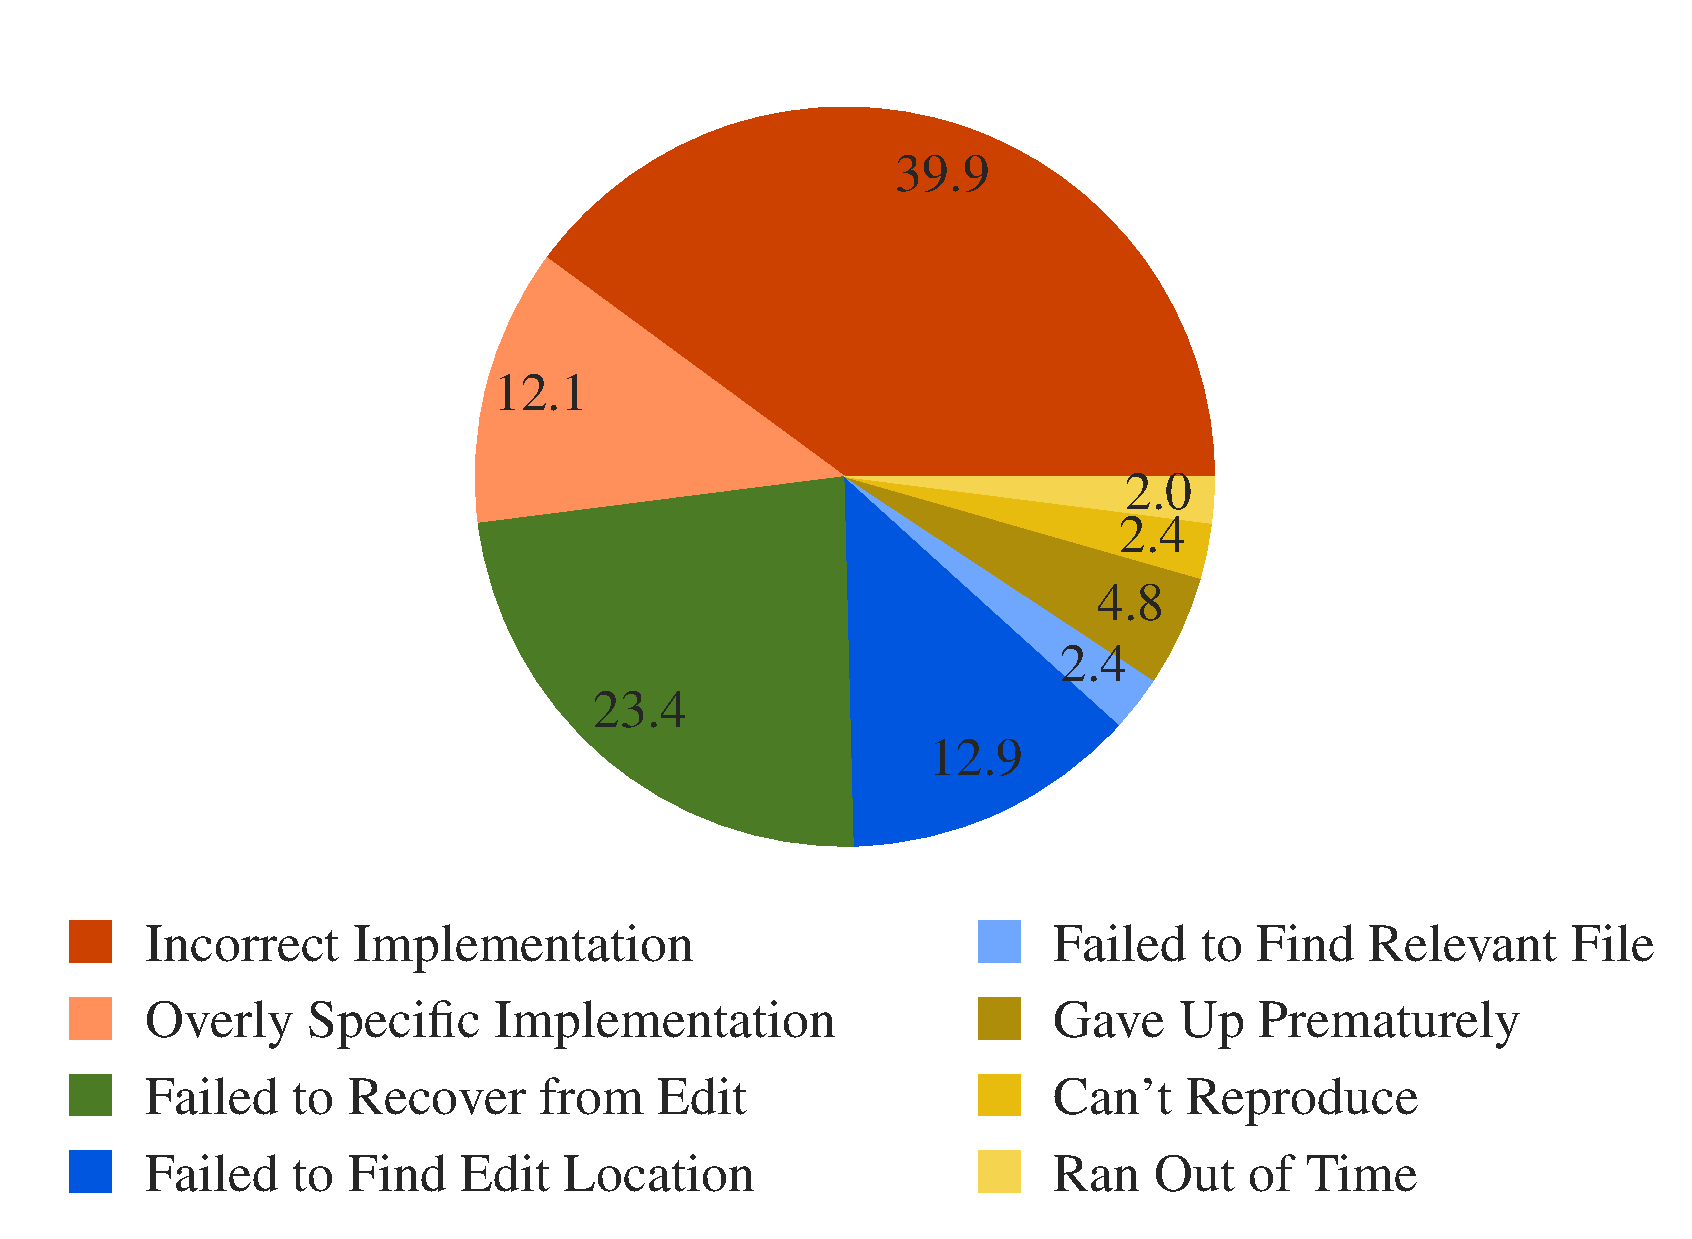
\includegraphics[width=\linewidth]{figures/failure_modes_pie.pdf}
    \caption{
    Failure mode distribution for SWE-agent w/ GPT-4 Turbo trajectories of unresolved instances.
    Each instance is labeled automatically using an LM with the categories from Table~\ref{tab:appx:failure_categories}.
    }
    \label{fig:failure_modes_pie}
  \end{minipage}
\end{figure}

\textbf{Agents succeed quickly and fail slowly.}
We find that runs submitted relatively early are much more likely to be successful compared to those submitted after a larger number of steps or cost.
We show in Table~\ref{fig:appx:steps_vs_cost_resolved} the distribution of resolved and unresolved instances, including only instances that did not exhaust their budget.
We observe that successful runs complete earlier and at a cheaper cost than unsuccessful ones. 
In general, successful instances solved by SWE-agent w/ GPT 4 finish with a median cost of \$\num{1.21} and \num{12} steps compared to a mean of \$\num{2.52} and \num{21} steps for unsuccessful ones.
Furthermore, we find that \num{93.0}\% of resolved instances are submitted before exhausting their cost budget, compared to \num{69.0}\% of instances overall.
For these reasons, we suspect that increasing the maximum budget or token limit are unlikely to substantially increase performance.
More statistics about how trajectories typically conclude are in \S\ref{appx:analyses:miscellaneous}.

\textbf{Most failures are incorrect implementations.}
We use GPT-4o to automatically categorize unresolved trajectories (SWE-agent w/ GPT-4 Turbo on SWE-bench Lite, $n=$\num{248}) into one of \num{9} manually defined categories described in Table~\ref{tab:appx:failure_categories}.
On a hand-labeled validation set, the LM's judgment agrees with the authors' on \num{87}\% of instances.
From Figure~\ref{fig:failure_modes_pie}, about half (\num{52.0}\%) of unresolved instances fall into the Incorrect Implementation or Overly Specific Implementation categories, suggesting that agents' proposed solutions often simply fail to functionally address the issue or are insufficiently general solutions.
Cascading failed edits make up another \num{23.4}\% of failures.
More details in \S\ref{appx:analyses:failure_modes}.